As I mentioned earlier I used three different sources and for the first source I used two different methods. 
\subsection{Electric Torch}
The first method used consists in making a continuous video through the large-angle lens contained in the mobile phone to be able to better visualize the first order of diffraction. Once the various processes explained in the previous section are finished, I extract the best frames from the video played by the sensor during the entire duration of the experiment, obtaining the following two images:
\begin{figure}[htp!]
  \centering
  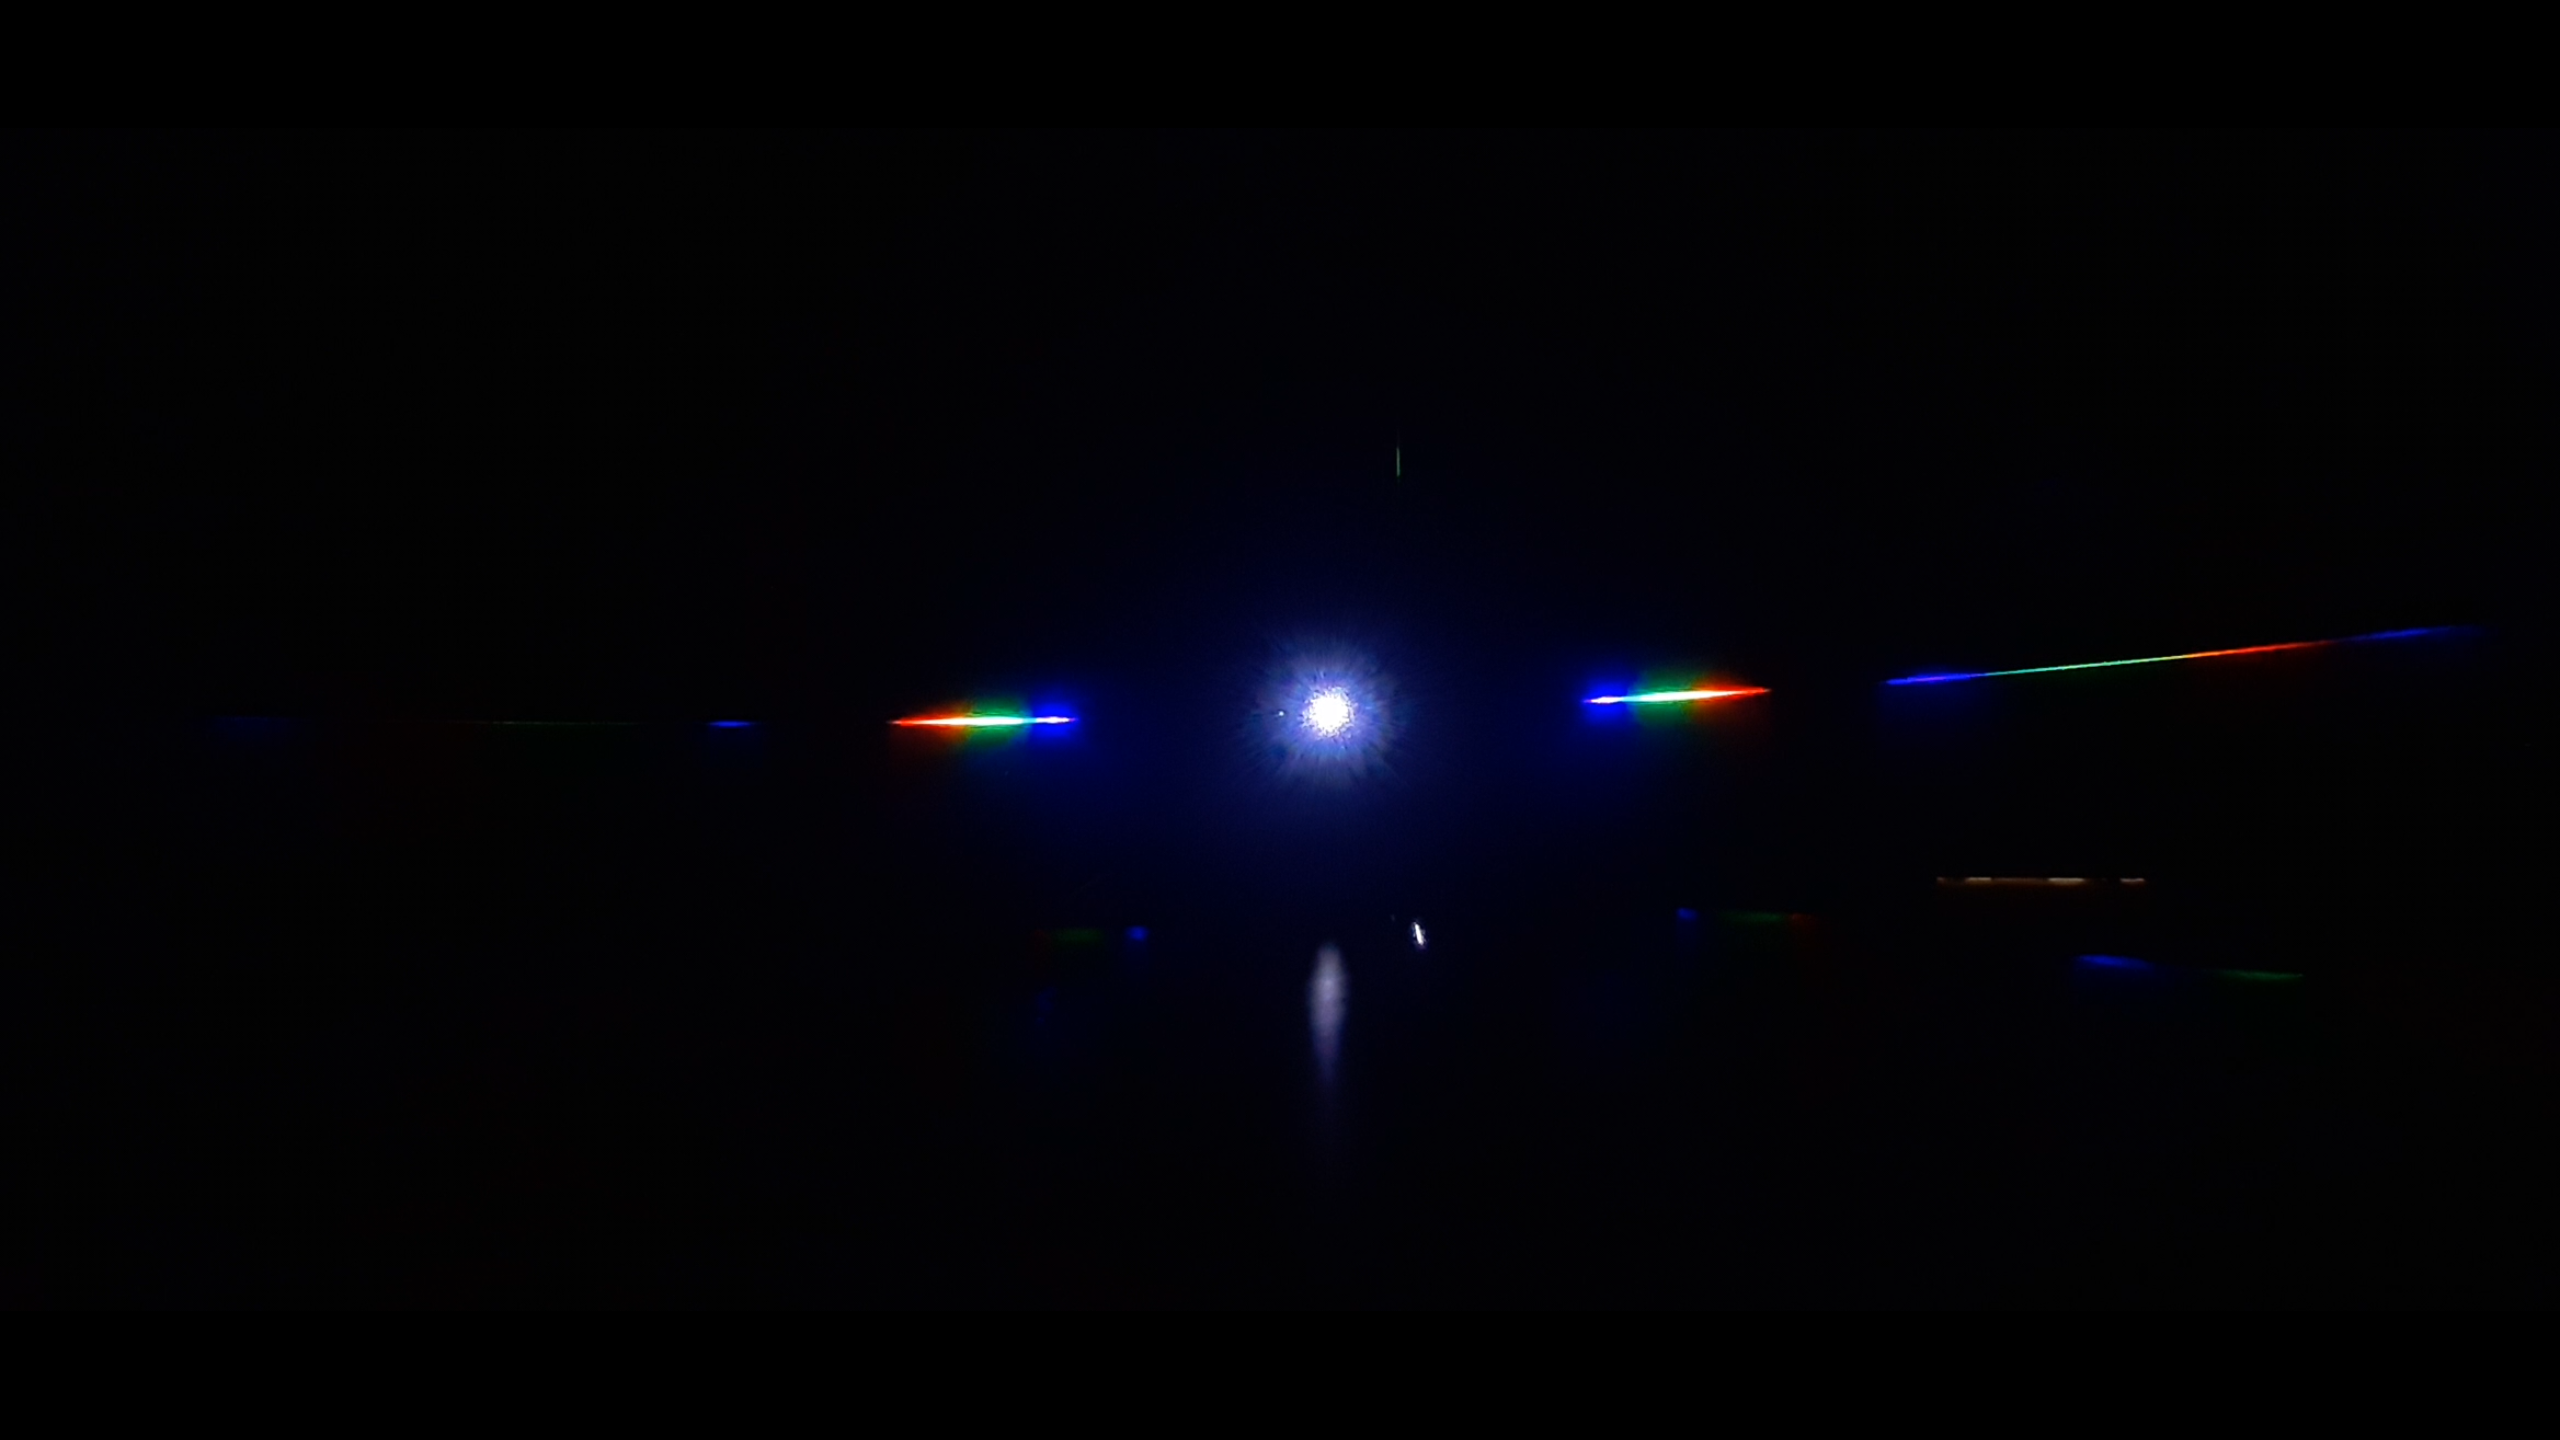
\includegraphics[scale=0.14]{Risultati Sperimentali/Primo reticoloT1.png} 
  \centering
  \qquad 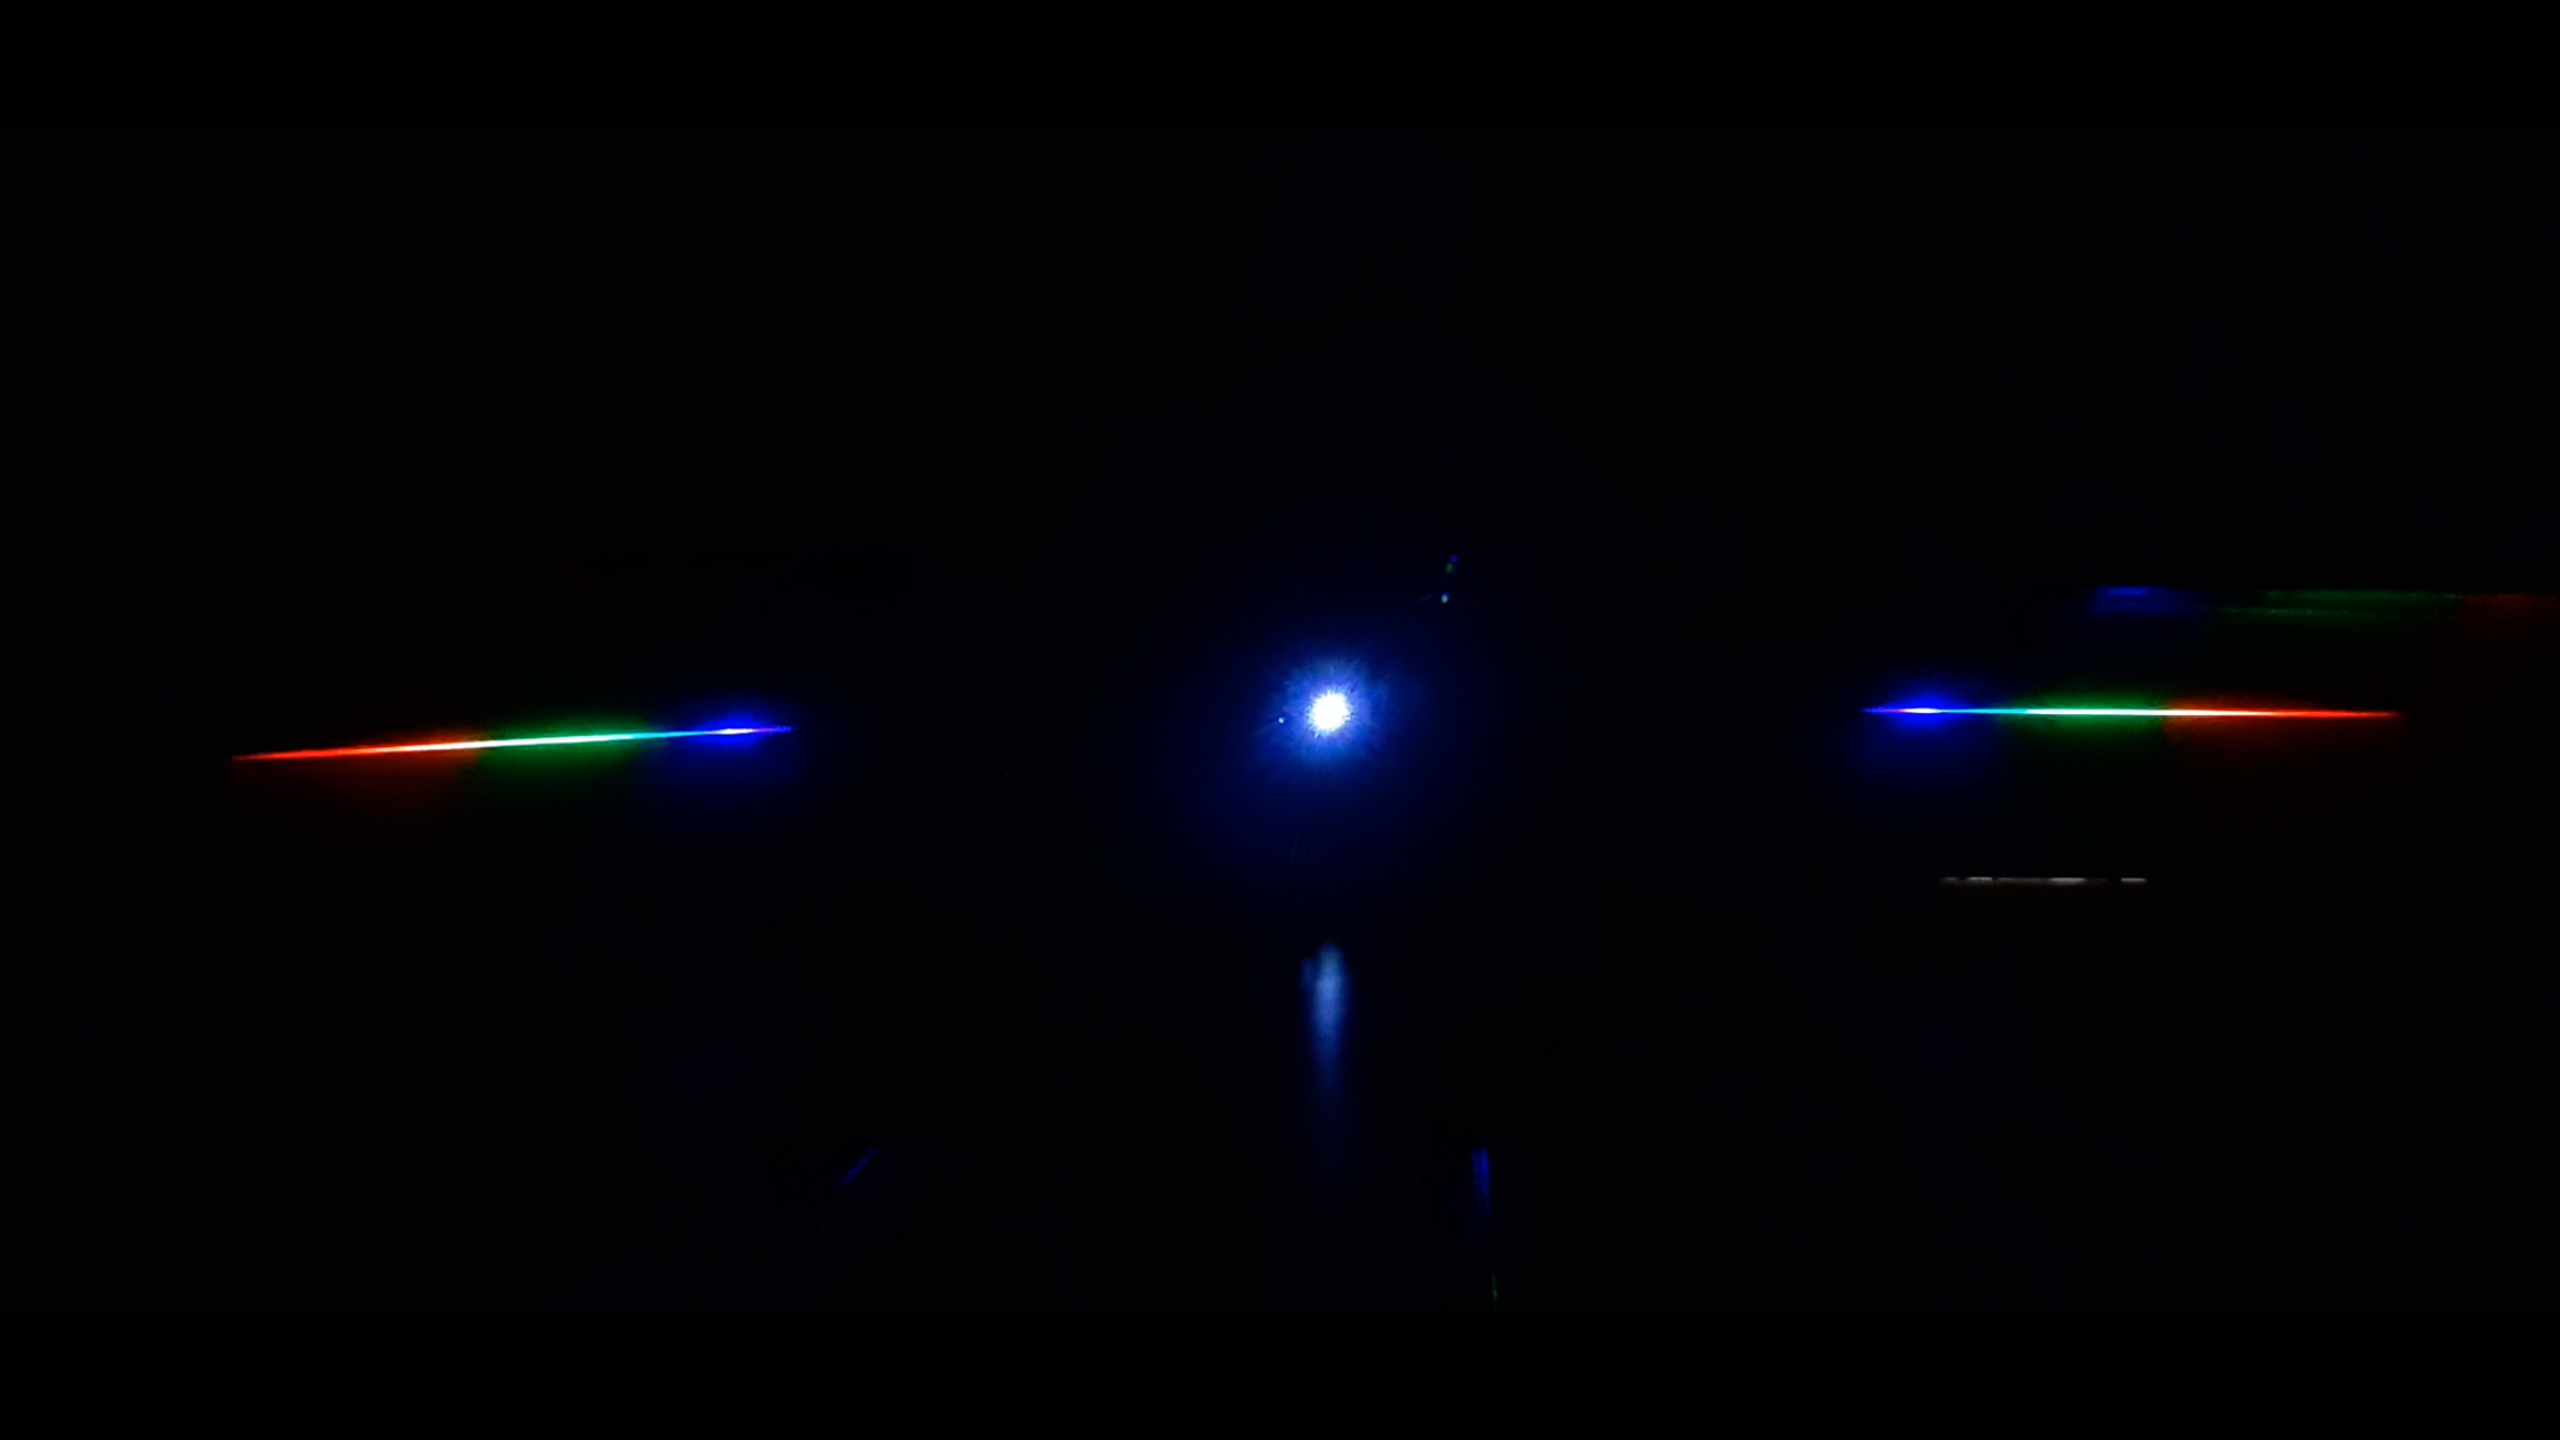
\includegraphics[scale=0.14]{Risultati Sperimentali/Secondo reticoloT1.png}
  \caption{In the first image it is possible to visualize the diffraction produced by the first holographic grating (with $d$ known) and in the second that produced by the second holographic grating (with $d'$ unknown). }
\end{figure}
\newpage
Obtaining the following results:
\begin{table}[ht!]
    \begin{tabular}{|c|c|c|c|c|c|}
    \hline
     $z\pm\sigma_z$ [mm] & $d$ [mm] & $\Delta x\pm\sigma_{\Delta x}$ [mm] & $\lambda\pm\sigma_\lambda$ [nm] & $\Delta x' \pm \sigma_{\Delta x'}$ [mm] & $d'\pm\sigma_{d'}$ [mm] \\
    \hline
    $4223\pm10$ & $0.002$ & $1093\pm15$ & $517.88\pm7.21$ & $2322\pm15$ & $(9.42\pm0.14)\times10^{-4}$ \\
    \hline
    \end{tabular}
    \caption{This table shows all the values with relative uncertainties measured and calculated during the first experience.}
\end{table}


The uncertainty related to $ d '$ was calculated through error propagation:
\begin{equation}
    \sigma_{d'}=\sqrt{\left(\frac{\lambda}{\Delta x}\right)^2\sigma_z^2+\left(\frac{\lambda z}{\Delta x'^2}\right)^2\sigma_{\Delta x'}^2+\left(\frac{z}{\Delta x}\right)^2\sigma_\lambda^2}
    \label{incertezza}
\end{equation}
Regarding the uncertainty $ \sigma_\lambda $ was obtained in a similar way using error propagation:
\begin{equation}
    \sigma_\lambda=\frac{\Delta x d}{z}
\end{equation}
For the uncertainty related to the measures of $ \Delta x $, $ \Delta x '$ and $ z $ they were chosen in a arbitrary way as it was difficult for me to quantify and calculate the error associated with these measures. For this reason I preferred to risk overestimating the error associated with direct measurements.
Ultimately getting $\text{liness/mm}=N$:
\begin{equation*}
    N=\frac{1}{d'}=(1061\pm17) \text{lines/mm}
\end{equation*}
I obtained the uncertainty related to lines/mm trhough error propagation:
\begin{equation}
    \sigma_N=\frac{1}{d'^2}\sigma_d'
\end{equation}
Using the second method without the wide-angle camera I obtained qualitatively consistent values:
\begin{table}[ht!]
    \begin{tabular}{|c|c|c|c|c|c|}
    \hline
     $z\pm\sigma_z$ [mm] & $d$ [mm] & $\Delta x\pm\sigma_{\Delta x}$ [mm] & $\lambda\pm\sigma_\lambda$ [nm] & $\Delta x' \pm \sigma_{\Delta x'}$ [mm] & $d'\pm\sigma_{d'}$ [mm] \\
    \hline
    $4223\pm10$ & $0.002$ & $985\pm15$ & $466.86\pm7.19$ & $2090\pm15$ & $(9.42\pm0.14)\times10^{-4}$ \\
    \hline
    \end{tabular}
    \caption{This table shows all the values with relative uncertainties measured and calculated during the first experience.}
\end{table}

From this I deduced that the wide angle does not modify the measurements taken in any way, you can view the images in the appendix.
\newpage
\subsection{First Bulb}
For the two bulbs I decided to change the measurement method: instead of making a continuous video and extracting the frames I decided to take single photos in the different configurations. These are the best images obtained by studying the first light bulb:
\begin{figure}[htp!]
  \centering
  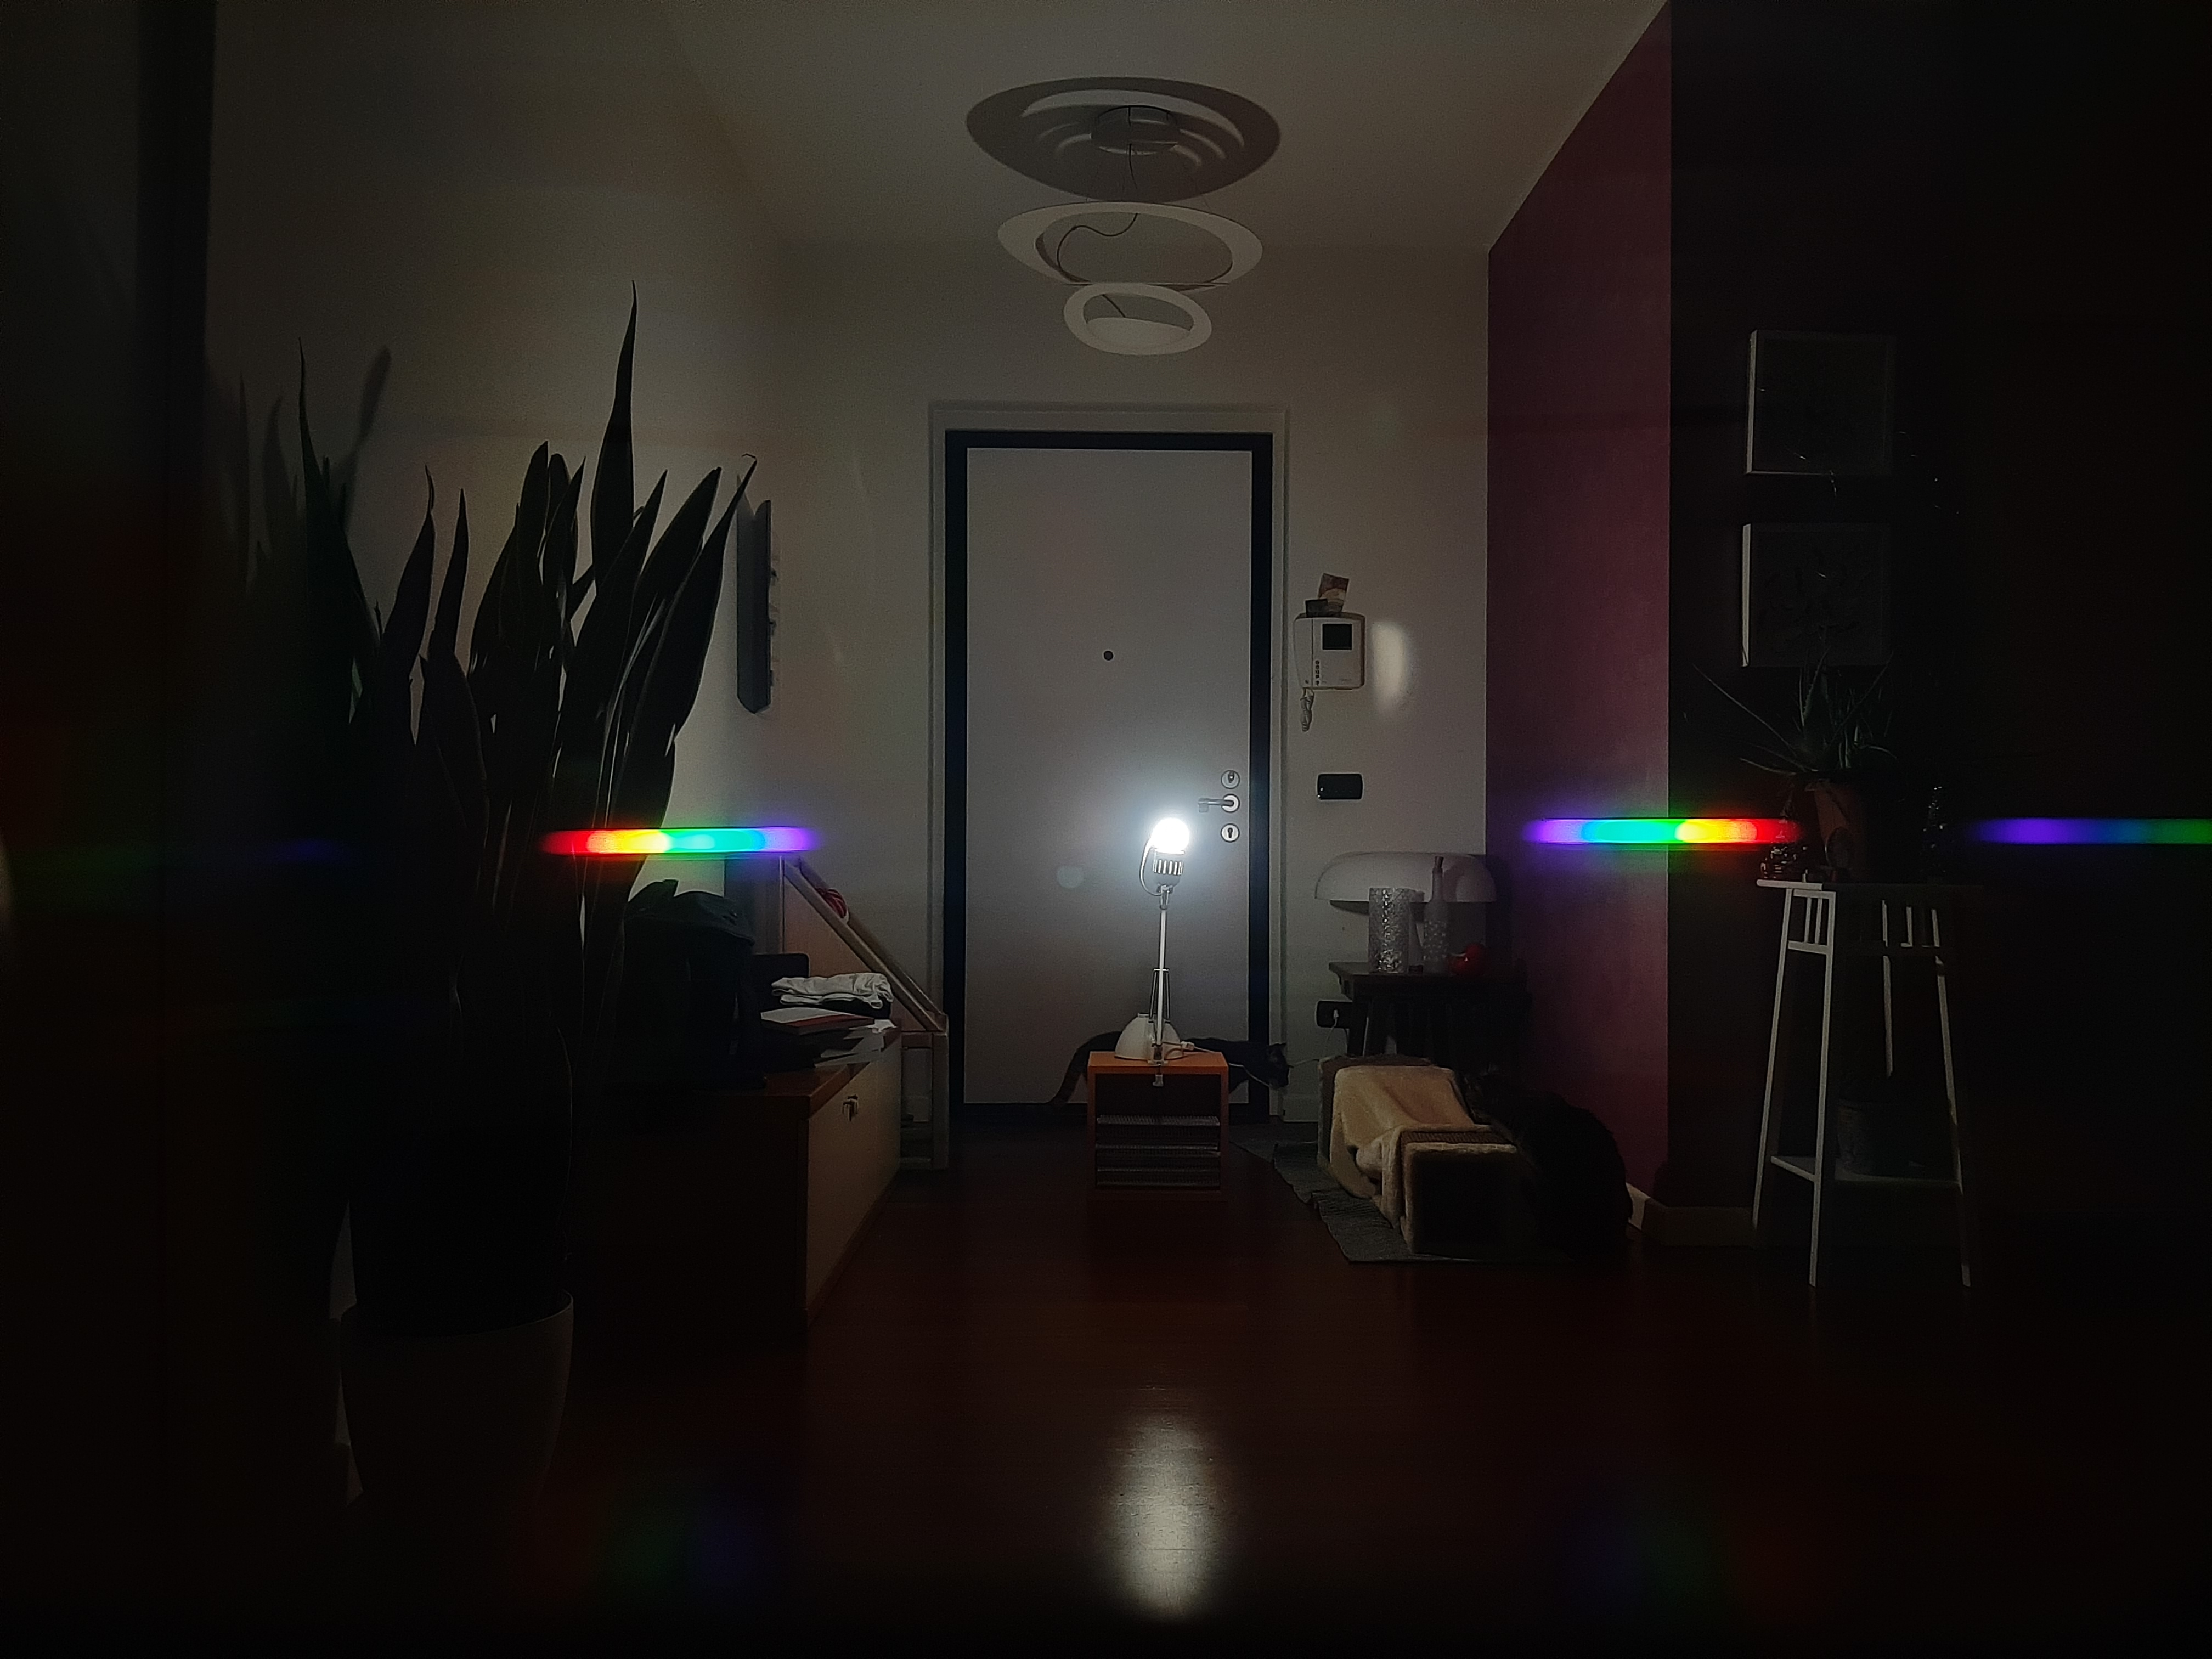
\includegraphics[scale=0.08]{Risultati Sperimentali/Lampada1a.jpg} 
  \centering
  \qquad 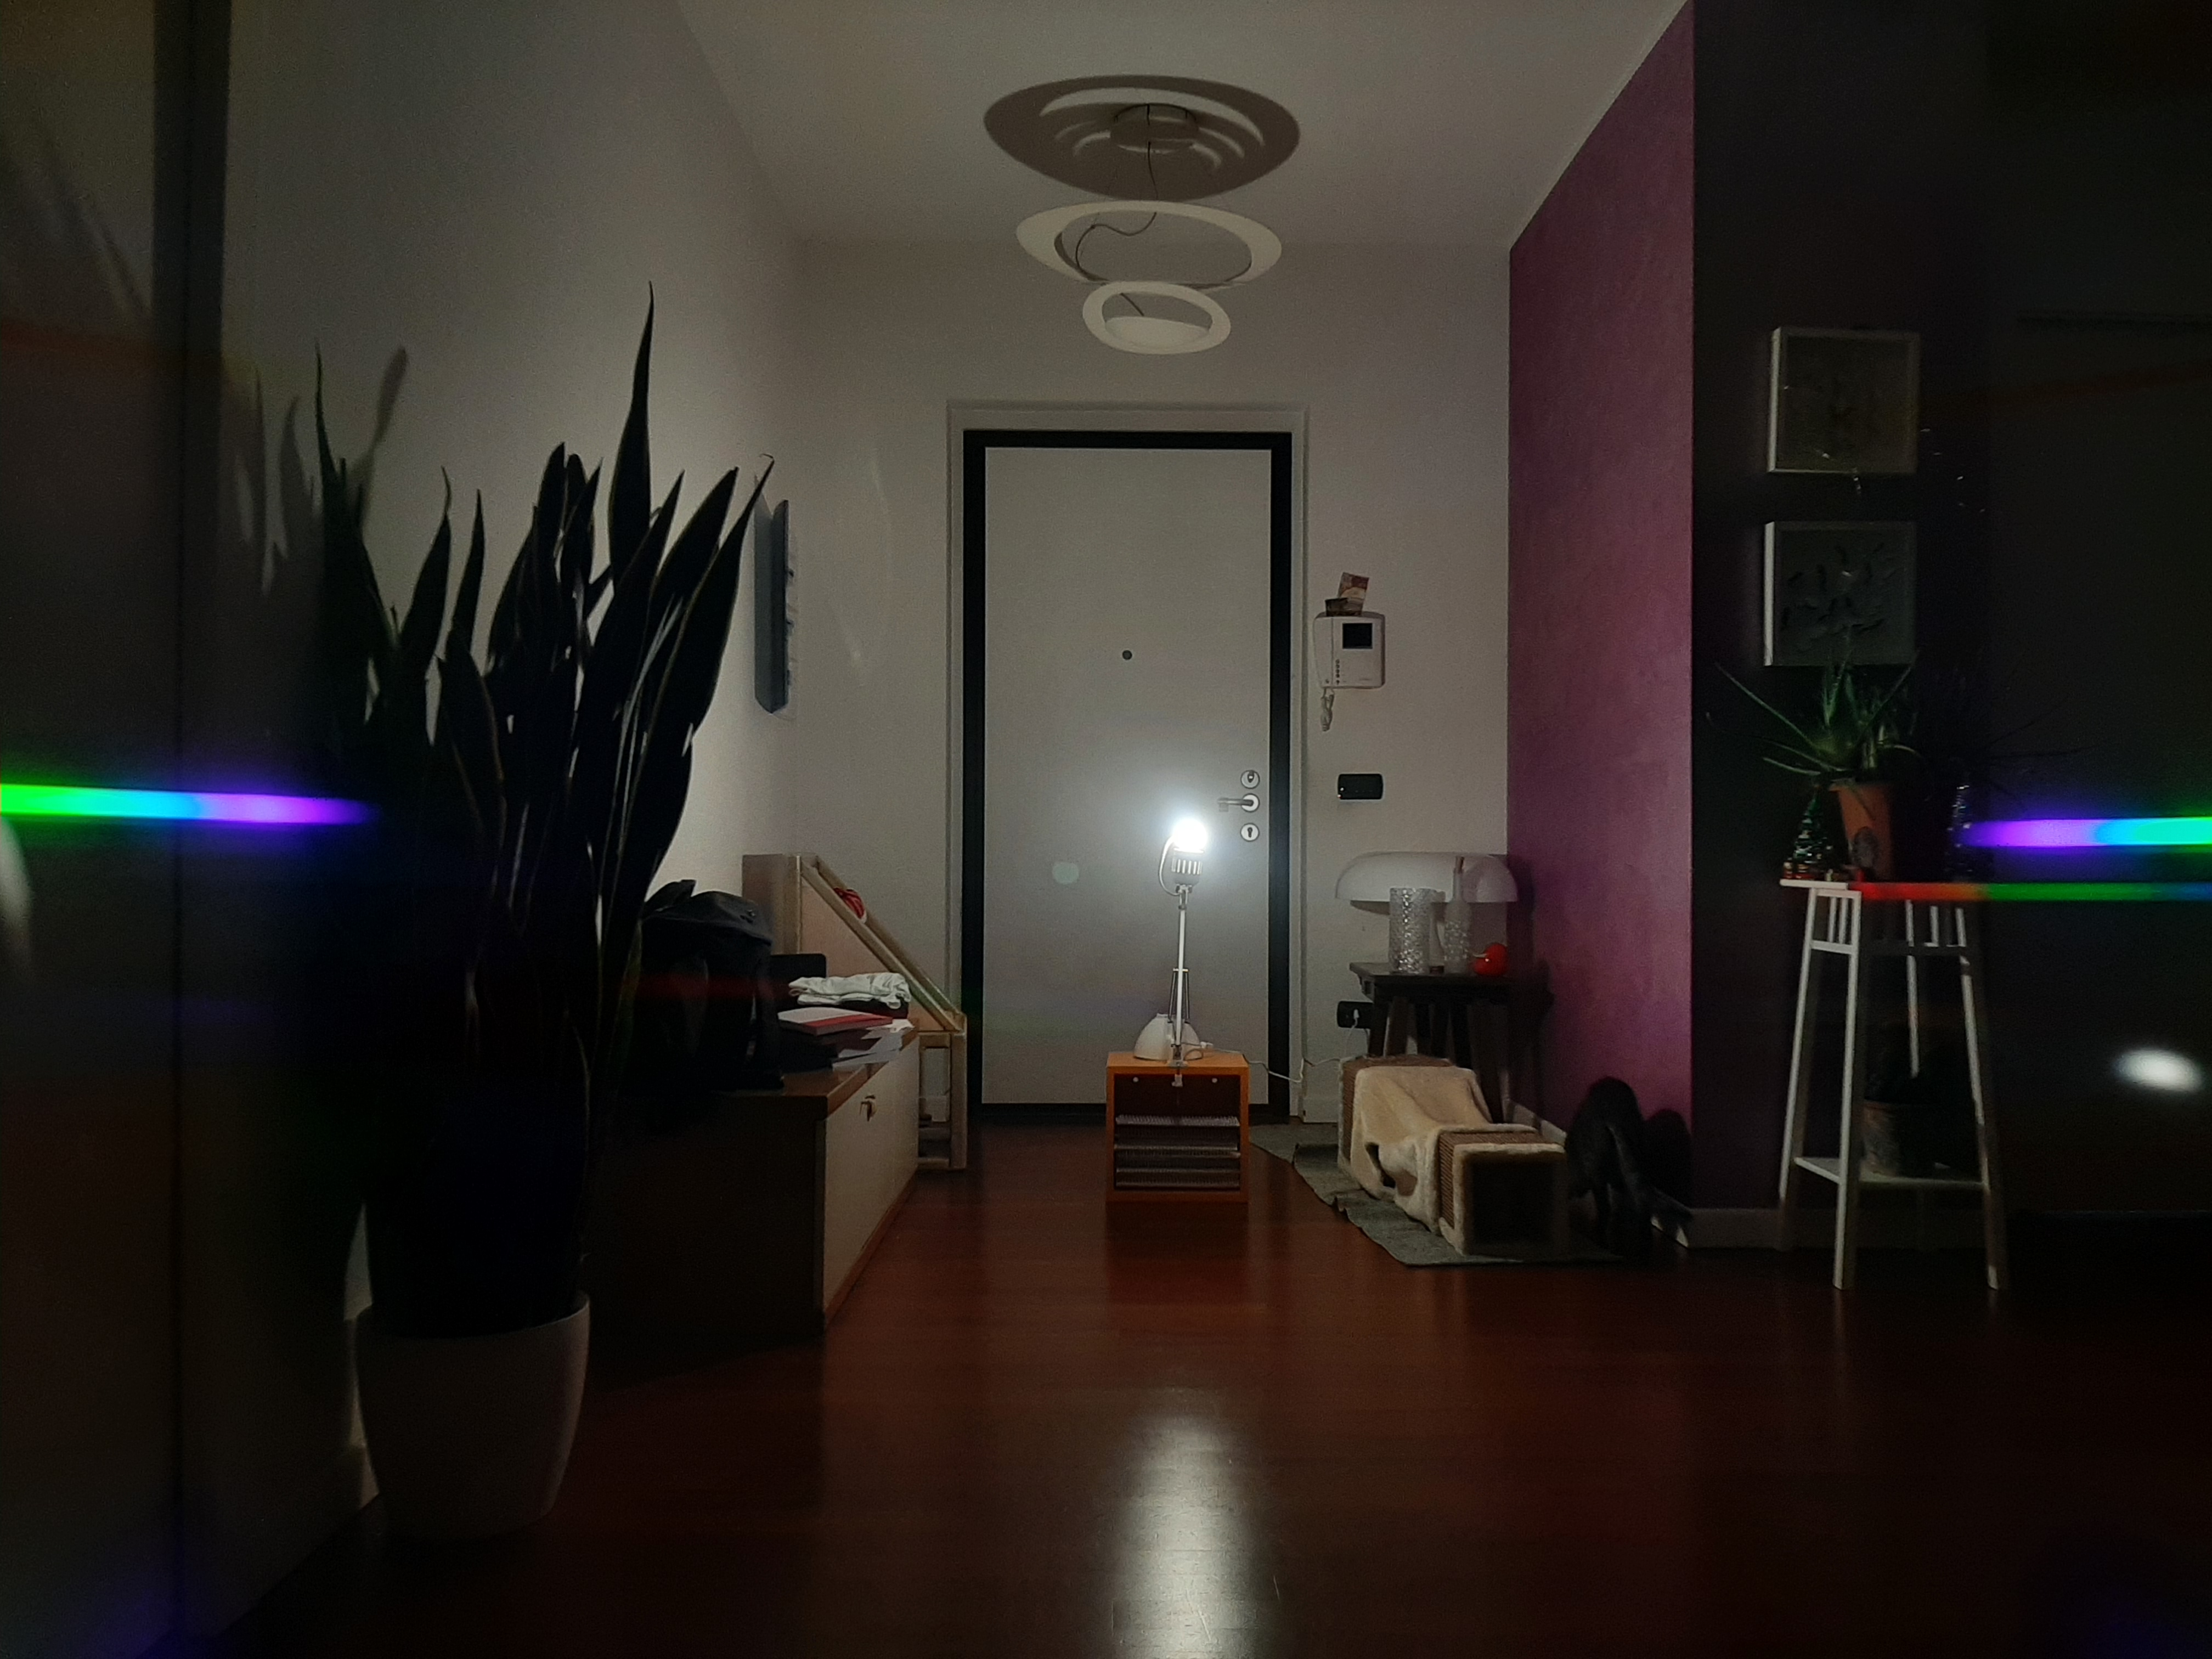
\includegraphics[scale=0.08]{Risultati Sperimentali/Lampada1b.jpg}
  \caption{In the first image it is possible to visualize the diffraction produced by the first holographic grating (with $d$ known) and in the second that produced by the second holographic grating (with $d'$ unknown). }
\end{figure}


Obtaining the following results shown in the table (\ref{t}).
\begin{table}[ht!]
    \begin{tabular}{|c|c|c|c|c|c|}
    \hline
     $z\pm\sigma_z$ [mm] & $d$ [mm] & $\Delta x\pm\sigma_{\Delta x}$ [mm] & $\lambda\pm\sigma_\lambda$ [nm] & $\Delta x' \pm \sigma_{\Delta x'}$ [mm] & $d'\pm\sigma_{d'}$ [mm] \\
    \hline
    $3730\pm10$ & $0.002$ & $1003\pm15$ & $538.05\pm8.17$ & $2180\pm15$ & $(9.20\pm0.16)\times10^{-4}$ \\
    \hline
    \end{tabular}
    \caption{This table shows all the values with relative uncertainties measured and calculated during the first experience.}
    \label{t}
\end{table}
The uncertainty relative to the value $d'$ is obtained through the equation (\ref{incertezza}) and therefore I obtained:
\begin{equation*}
    N=\frac{1}{d'}=(1086\pm18) \text{lines/mm}
\end{equation*}
\subsection{Second bulb}
These are the images I got by studying the second bulb (warm light):
\begin{figure}[htp!]
  \centering
  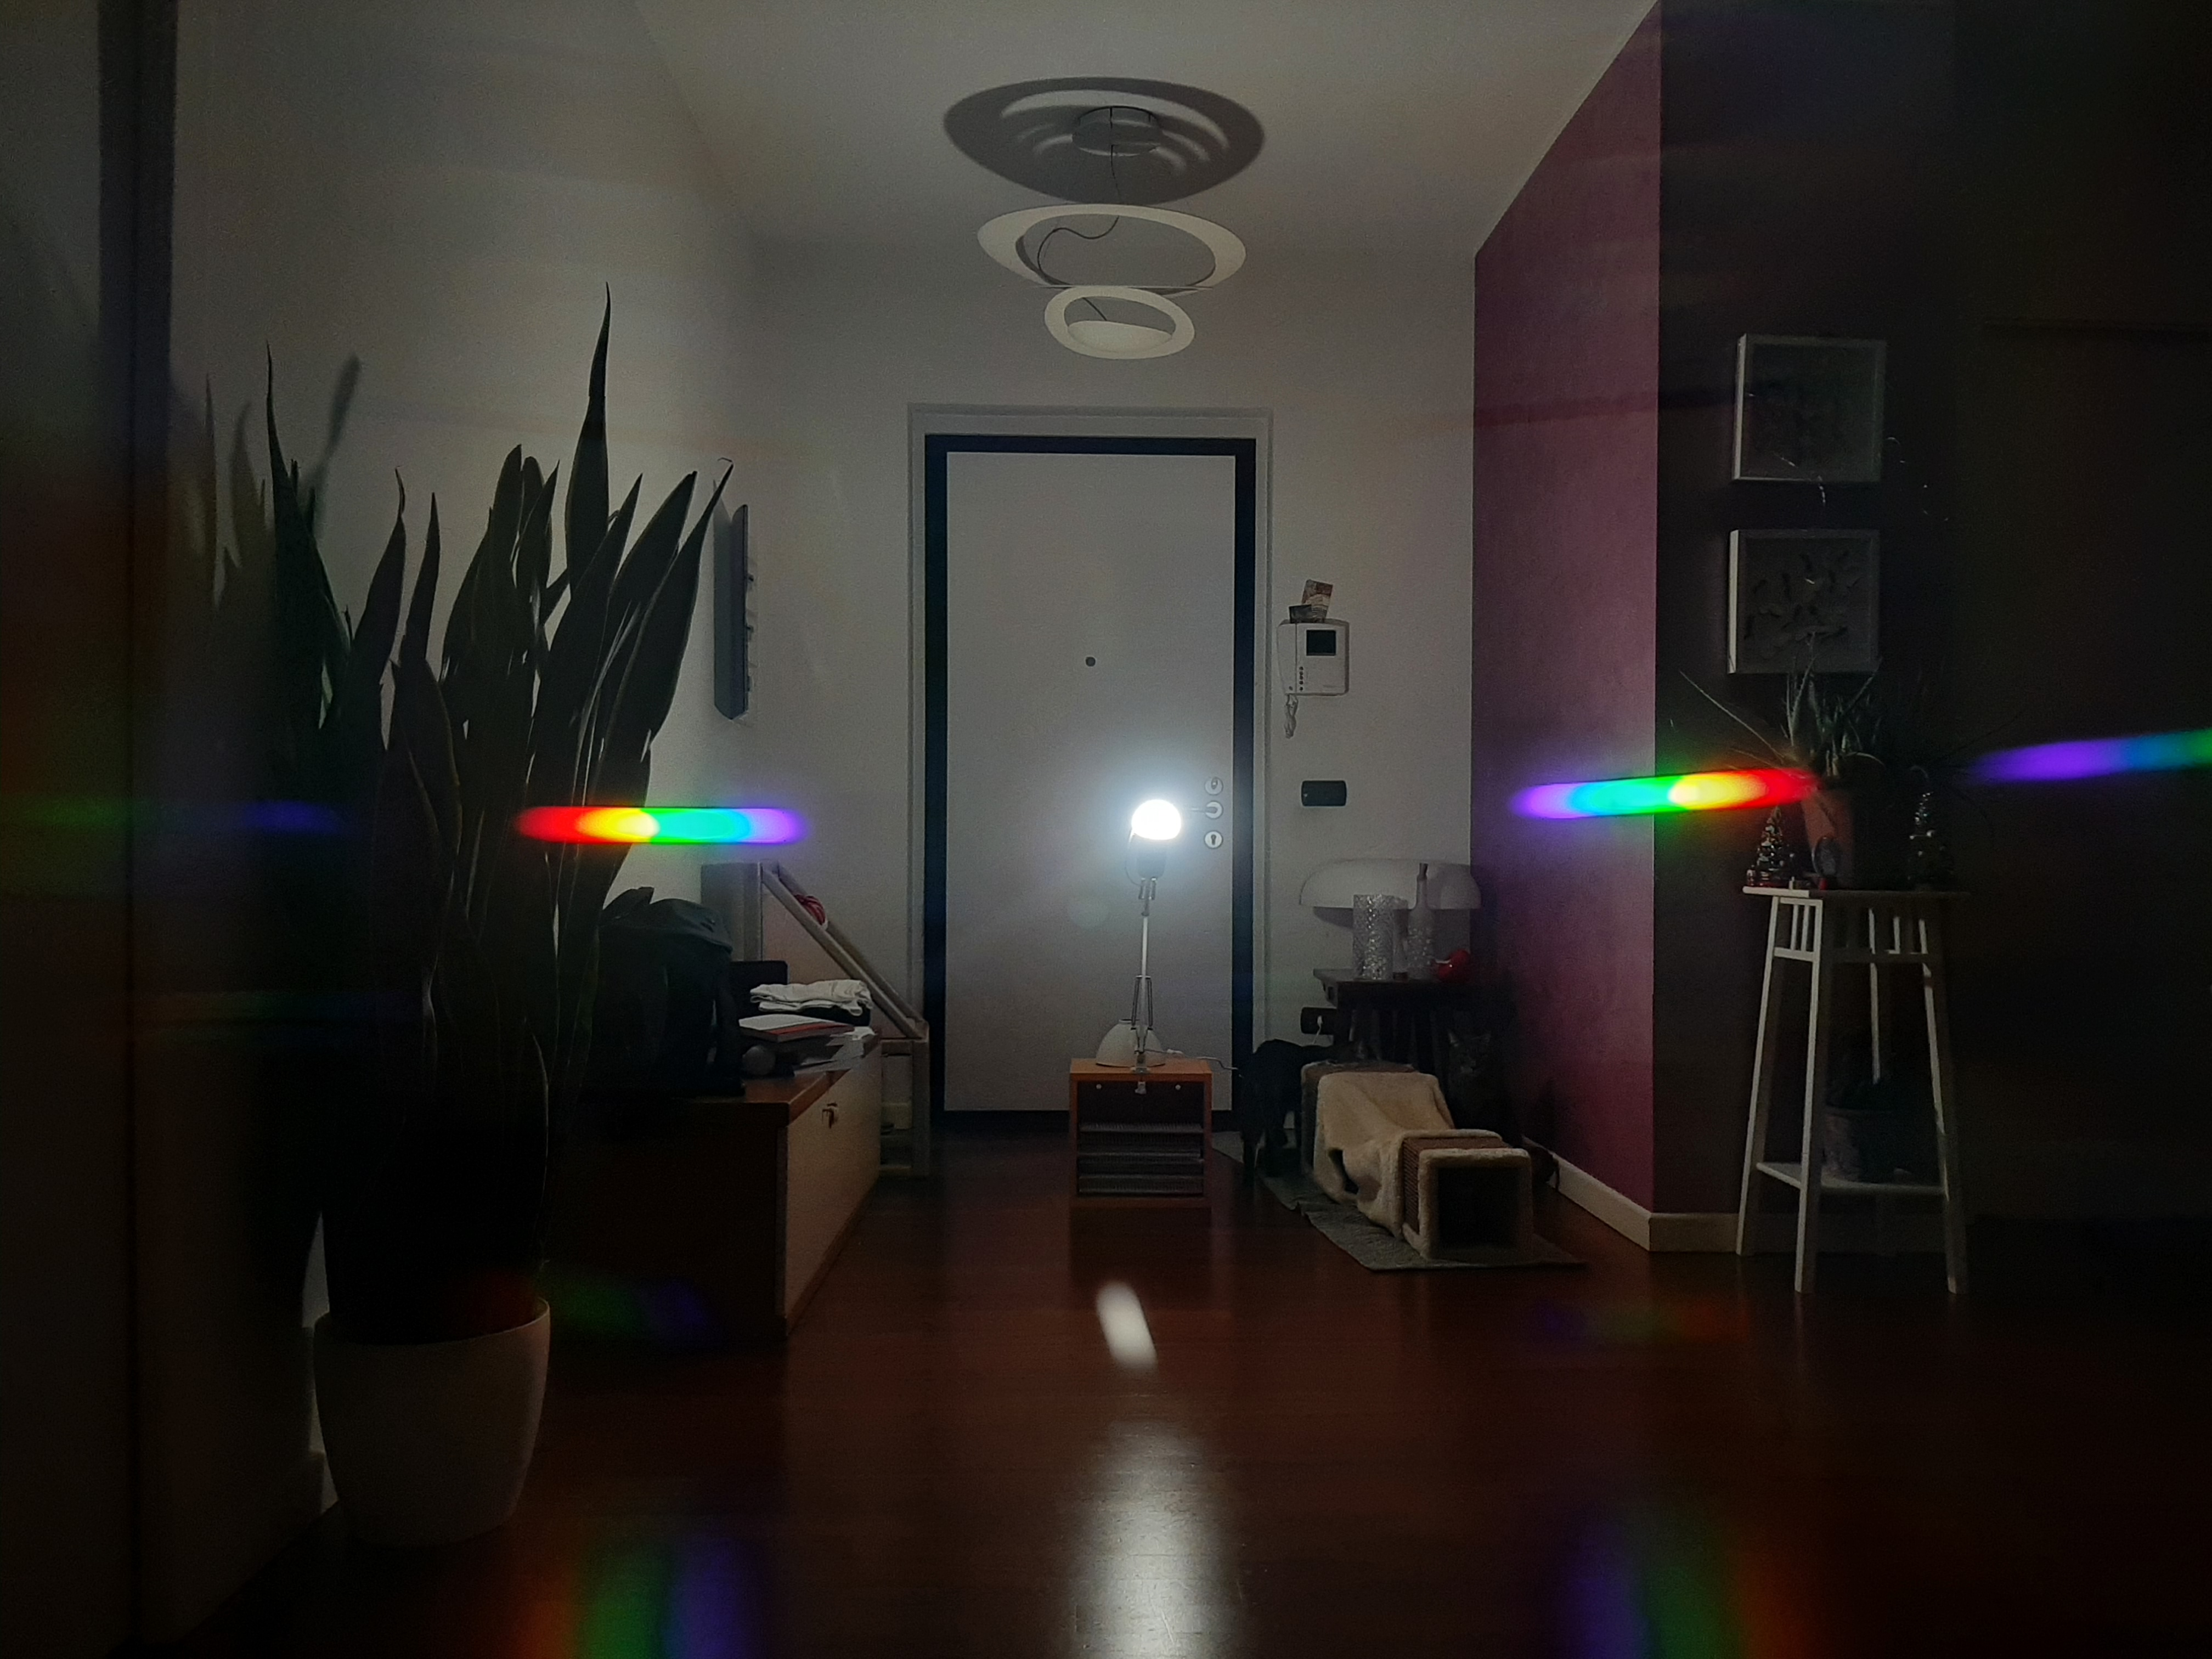
\includegraphics[scale=0.08]{Risultati Sperimentali/Lampada2a.jpg} 
  \centering
  \qquad 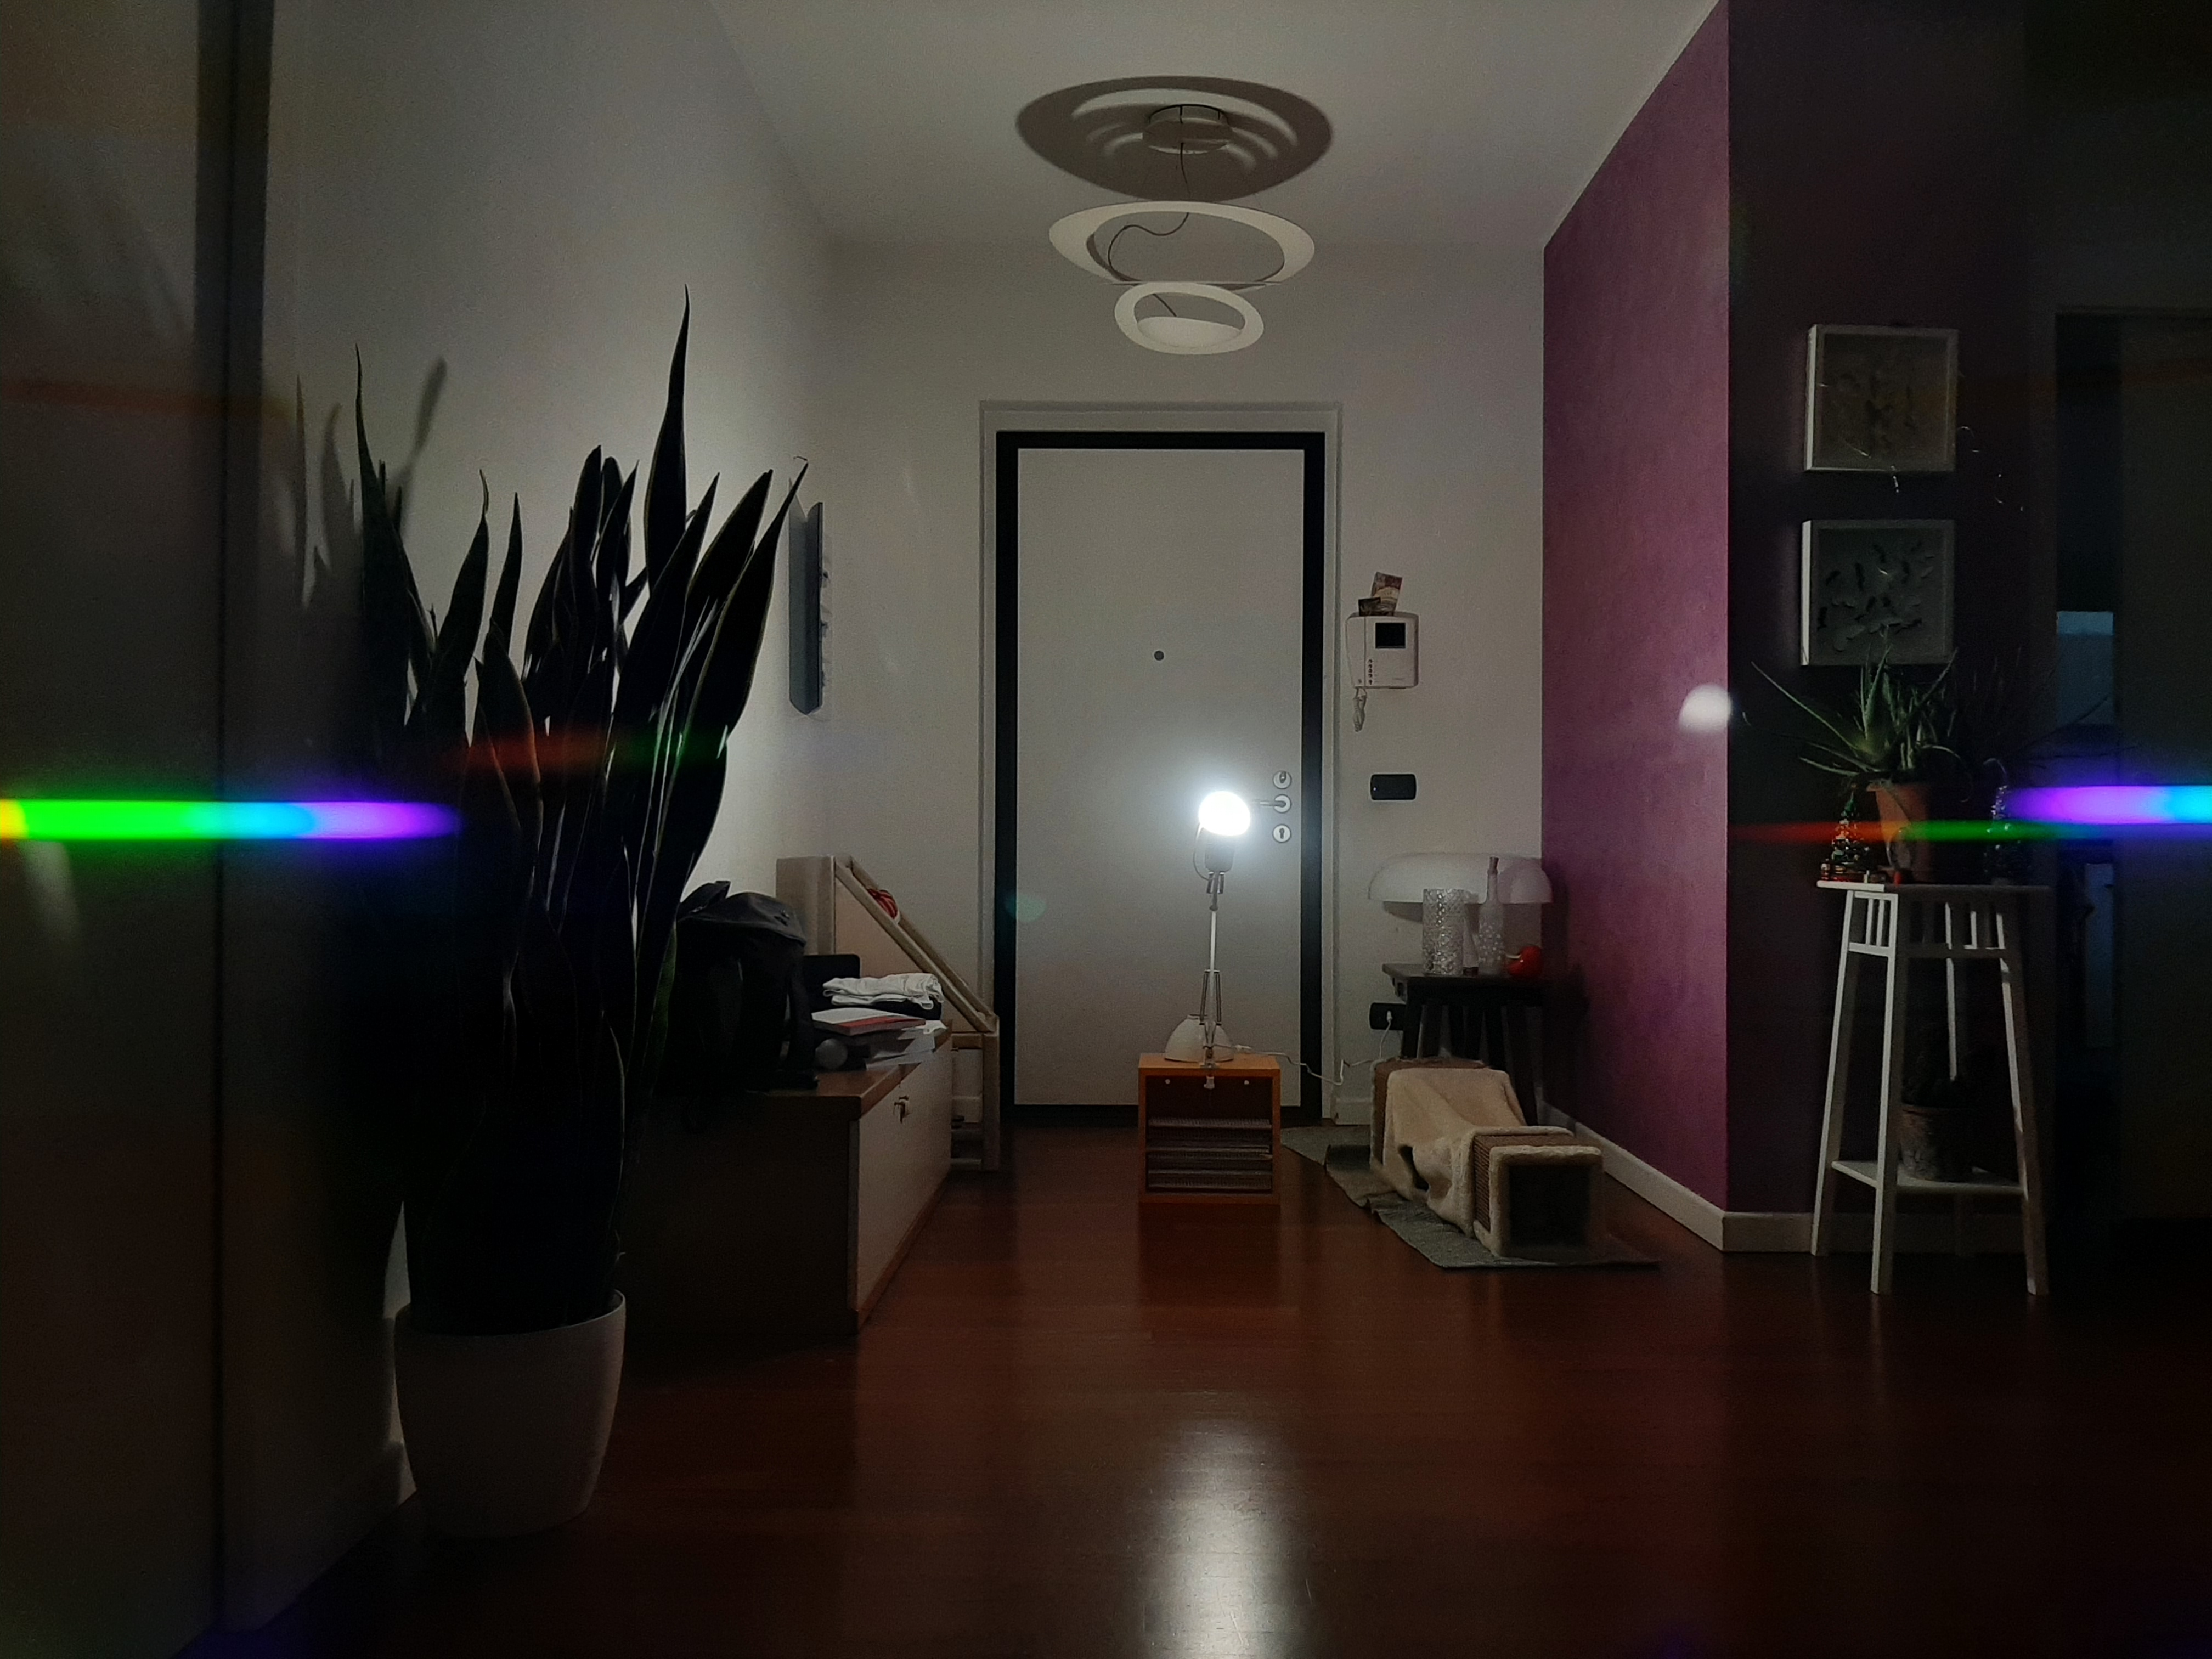
\includegraphics[scale=0.08]{Risultati Sperimentali/Lampada2b.jpg}
  \caption{In the first image it is possible to visualize the diffraction produced by the first holographic grating (with $d$ known) and in the second that produced by the second holographic grating (with $d'$ unknown). }
\end{figure}
\newpage
Obtaining the following results:
\begin{table}[ht!]
    \begin{tabular}{|c|c|c|c|c|c|}
    \hline
     $z\pm\sigma_z$ [mm] & $d$ [mm] & $\Delta x\pm\sigma_{\Delta x}$ [mm] & $\lambda\pm\sigma_\lambda$ [nm] & $\Delta x' \pm \sigma_{\Delta x'}$ [mm] & $d'\pm\sigma_{d'}$ [mm] \\
    \hline
    $3730\pm10$ & $0.002$ & $993\pm15$ & $532.97\pm8.17$ & $2126\pm15$ & $(9.34\pm0.16)\times10^{-4}$ \\
    \hline
    \end{tabular}
    \caption{This table shows all the values with relative uncertainties measured and calculated during the first experience.}
\end{table}


The uncertainty relative to the value $d'$ is obtained through the equation (\ref{incertezza}) and therefore I obtained:
\begin{equation*}
    N=\frac{1}{d'}=(1069\pm18) \text{lines/mm}
\end{equation*}
